%% LyX 2.2.4 created this file.  For more info, see http://www.lyx.org/.
%% Do not edit unless you really know what you are doing.
\documentclass[english]{article}
\usepackage[T1]{fontenc}
\usepackage[latin9]{inputenc}
\usepackage{geometry}
\geometry{verbose,lmargin=25mm,rmargin=25mm}
\usepackage{amsmath}
\usepackage{amssymb}
\usepackage{graphicx}
\usepackage{babel}
\begin{document}

\title{Weak localization in Hydrogenated Graphene}
\maketitle

\section{Introduction}

\subsection{Weak localization}

\section{Tight-binding model}

To explore this system we are going to adopt a tight-binding formulation
given by the reference {[}PRL 110, 246602(2013){]}. Basically our
model can be splitted in two parts: an orbital and a spin-orbit couping
part,

\begin{equation}
H=H_{\text{orb}}+H_{\text{so}}\label{eq:Hamiltonian_general}
\end{equation}
In what follows we have adopted the notation where $c_{i\sigma}^{\dagger}=(a_{i\sigma}^{\dagger},b_{i\sigma}^{\dagger})$
and $c_{i\sigma}=(a_{i\sigma},b_{i\sigma})$ represent the creation
and annihilation operators for the $p_{z}$-orbitals on both A and
B graphene sublattices. The creation and annihilation operators for
the Hydrogen $s$-orbitals located at the site $m$ are given respectivelly
by $h_{m\sigma}^{\dagger}$ and $h_{m\sigma}$. The orbital part of
\ref{eq:Hamiltonian_general} is given by 

\begin{equation}
H_{\text{orb}}=\varepsilon_{h}\sum_{m}h_{m\sigma}^{\dagger}h_{m\sigma}-t\sum_{\langle i,j\rangle}c_{i\sigma}^{\dagger}c_{j\sigma}+T\sum_{\langle m,i\rangle}h_{m\sigma}^{\dagger}c_{i\sigma}+\text{\text{h.c}.}
\end{equation}
where 
\begin{itemize}
\item $\varepsilon_{h}=3$ eV is the adatom on-site energy, which could
be fitted from first-principles band structure for $\Delta/a=14\%$
(distortion in the single-adatom limit).
\item $T=6.5$ eV is the Hydrogen-Carbon hopping term, which was also obtained
by fitting.
\item $t=2.6$ eV, is the hopping term between the Carbon atoms, Ref.'s
{[}30{]} and {[}36{]} os PRL 110, 246602(2013).
\end{itemize}
The spin-orbit coupling part can be written as

\[
H_{\text{so}}=\frac{2i}{3}\sum_{\langle i,j\rangle}c_{i\sigma}^{\dagger}c_{j\sigma^{\prime}}\left[\Lambda_{\text{BR}}(\mathbf{s}\times\mathbf{d}_{ij})\right]_{\sigma\sigma^{\prime}}+\frac{i}{3}\sum_{\langle\langle i,j\rangle\rangle}c_{i\sigma}^{\dagger}c_{j\sigma}\left[\frac{\Lambda_{I}^{c}}{\sqrt{3}}\nu_{ij}\hat{s}_{z}+2\Lambda_{\text{PIA}}^{c}(\mathbf{s}\times\mathbf{D}_{ij})_{z}\right]_{\sigma\sigma^{\prime}}
\]
where
\begin{itemize}
\item $\Lambda_{\text{BR}}$: Bychkov-Rashba term
\item $\Lambda_{I}^{A}$, $\Lambda_{I}^{B}$: intrinsic SOC, which depends
on the sublattice
\item $\Lambda_{\text{PIA}}^{A}$, $\Lambda_{\text{PIA}}^{B}$: new SOC
due to pseudospin inversion asymmetry
\item $\nu_{ij}=1$ for counter-clockwise path from $j$ to $i$
\item $\nu_{ij}=-1$ for clockwise path from $j$ to $i$
\item $\mathbf{d}_{ij}$: nearest-neighbor unit vector from $j$ to $i$
\item $\mathbf{D}_{ij}$: next-nearest-neighbor unit vector from $j$ to
$i$
\end{itemize}

\subsection{Single-adatom limit}

In this case, the minimal realistic model for SOC has its effects
confined up to the second-nearest neighbors of the hydronated site
$C_{H}$ (in sublattice A), which defines our impurity region. Defining
$A_{\sigma}^{\dagger}$ $(A_{\sigma})$ as the creation (annihilation)
operator on $C_{H}$ and $B_{m\sigma}^{\dagger}$ $(B_{m\sigma})$
as the creation (annihilation) operator on the three nearest neighbors
of $C_{H}$. The tight-binding Hamiltonian can be written as

\begin{align*}
H_{\text{so}} & =\frac{i}{3}\sum_{\langle\langle i,j\rangle\rangle}^{\prime}c_{i\sigma}^{\dagger}c_{j\sigma^{\prime}}\left[\frac{\lambda_{I}}{\sqrt{3}}\nu_{ij}\hat{s}_{z}\right]_{\sigma\sigma^{\prime}}\\
 & +\frac{i}{3}\sum_{\langle\langle C_{H},j\rangle\rangle}A_{\sigma}^{\dagger}c_{j\sigma^{\prime}}\left[\frac{\Lambda_{I}}{\sqrt{3}}\nu_{C_{H},j}\hat{s}_{z}\right]_{\sigma\sigma^{\prime}}\\
 & +\frac{2i}{3}\sum_{\langle C_{H},j\rangle}A_{\sigma}^{\dagger}B_{j\sigma^{\prime}}\left[\Lambda_{\text{BR}}(\hat{\mathbf{s}}\times\mathbf{d}_{C_{H},j})_{z}\right]_{\sigma\sigma^{\prime}}+\text{h.c.}\\
 & +\frac{2i}{3}\sum_{\langle\langle i,j\rangle\rangle}B_{i\sigma}^{\dagger}B_{j\sigma^{\prime}}\left[\Lambda_{\text{PIA}}(\hat{\mathbf{s}}\times\mathbf{D}_{i,j})_{z}\right]_{\sigma\sigma^{\prime}}
\end{align*}
where the individual terms and parameters assume the following interpretation
and values:
\begin{itemize}
\item The first term models the intrinsic spin-orbit coupling for the Graphene,
and it is characterized by $2\lambda_{I}=24$ $\mu$eV. It couples
every next-nearest-neighbor pairs that do not contain $C_{H}$ (indicated
by the prime).
\item The second term indicates the adatom-induced intrinsic SOC, and it's
strength is given by $\Lambda_{I}=-0.21$ meV (17 times stronger than
$\lambda_{I}$). It couples the same spin in the same sublattice.
\item The third term is the Bychkov-Rashba term, which induces the nearest
neighbors spin-flip. The value of $\Lambda_{\text{BR}}=0.33$ meV
is more than 60 times stronger than the value for Graphene in a representative
electric field of $1$ V/nm ($\lambda_{\text{BR}}=5$ $\mu$eV).
\item The last term comes from the pseudo-spin asymmetry and couples different
spin from next-nearest-neighbors. The value of $\Lambda_{\text{PIA}}=-0.77$
meV has no couterpart in flat Graphene.
\end{itemize}

\section{Preliminar results}

The main subject of this study is a two-dimensional strip of Graphene
with Hydrogen adatoms in one side of the strip. To start the investigation,
let us focus on a simple Graphene strip as depicted in the figure
(\ref{fig:Zig-zag-Graphene-strip}).

\begin{figure}
\begin{centering}
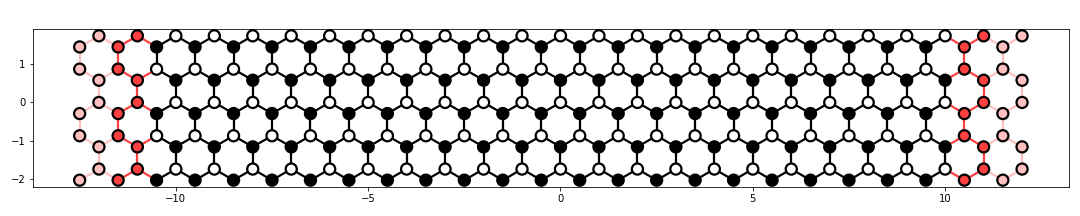
\includegraphics[viewport=0cm 0bp 1080bp 360bp,clip,width=0.8\columnwidth]{/home/marcos/Documents/DAAD_Research/quantum_transport/hydrogenated_graphene/images/Graphene_strip_example}
\par\end{centering}
\caption{Zig-zag Graphene strip connected to semi-infinite leads on the left
and on the right.\label{fig:Zig-zag-Graphene-strip}}
\end{figure}

To introduxe an out-of-plane magnetic field into our system, we have
implemented the Peierls substitution, where the original hoppings
are replaced by 

\begin{equation}
t_{i,j}\rightarrow t_{i,j}e^{i\phi_{ij}}
\end{equation}
where the Peierls phase is defined by

\begin{equation}
\phi_{ij}=\frac{e}{\hbar}\int_{\mathbf{r}_{i}}^{\mathbf{r}_{j}}\mathbf{A}\cdot d\mathbf{l}
\end{equation}
with $\mathbf{A}$ being the vector potential, and $\mathbf{r}_{i}$
the position of the i-th atom. To get a zero magnetic field in the
leads, and a magnetic field pointing in z-direction we adopt the Landau
gauge given by

\begin{equation}
\mathbf{A}(\mathbf{r})=\hat{\mathbf{y}}B\bar{x}
\end{equation}

\begin{equation}
\bar{x}=\begin{cases}
\begin{array}{c}
0,\\
x,\\
d,
\end{array} & \begin{array}{c}
x<0\\
0\leq x\leq d\\
x>d
\end{array}\end{cases}.
\end{equation}

Notice that the vector potential can not be set to zero in the $x>d$
region, as this would imply an infinite magnetic field at the $x=d$
interface.

\section{Results}

\begin{figure}
\begin{centering}
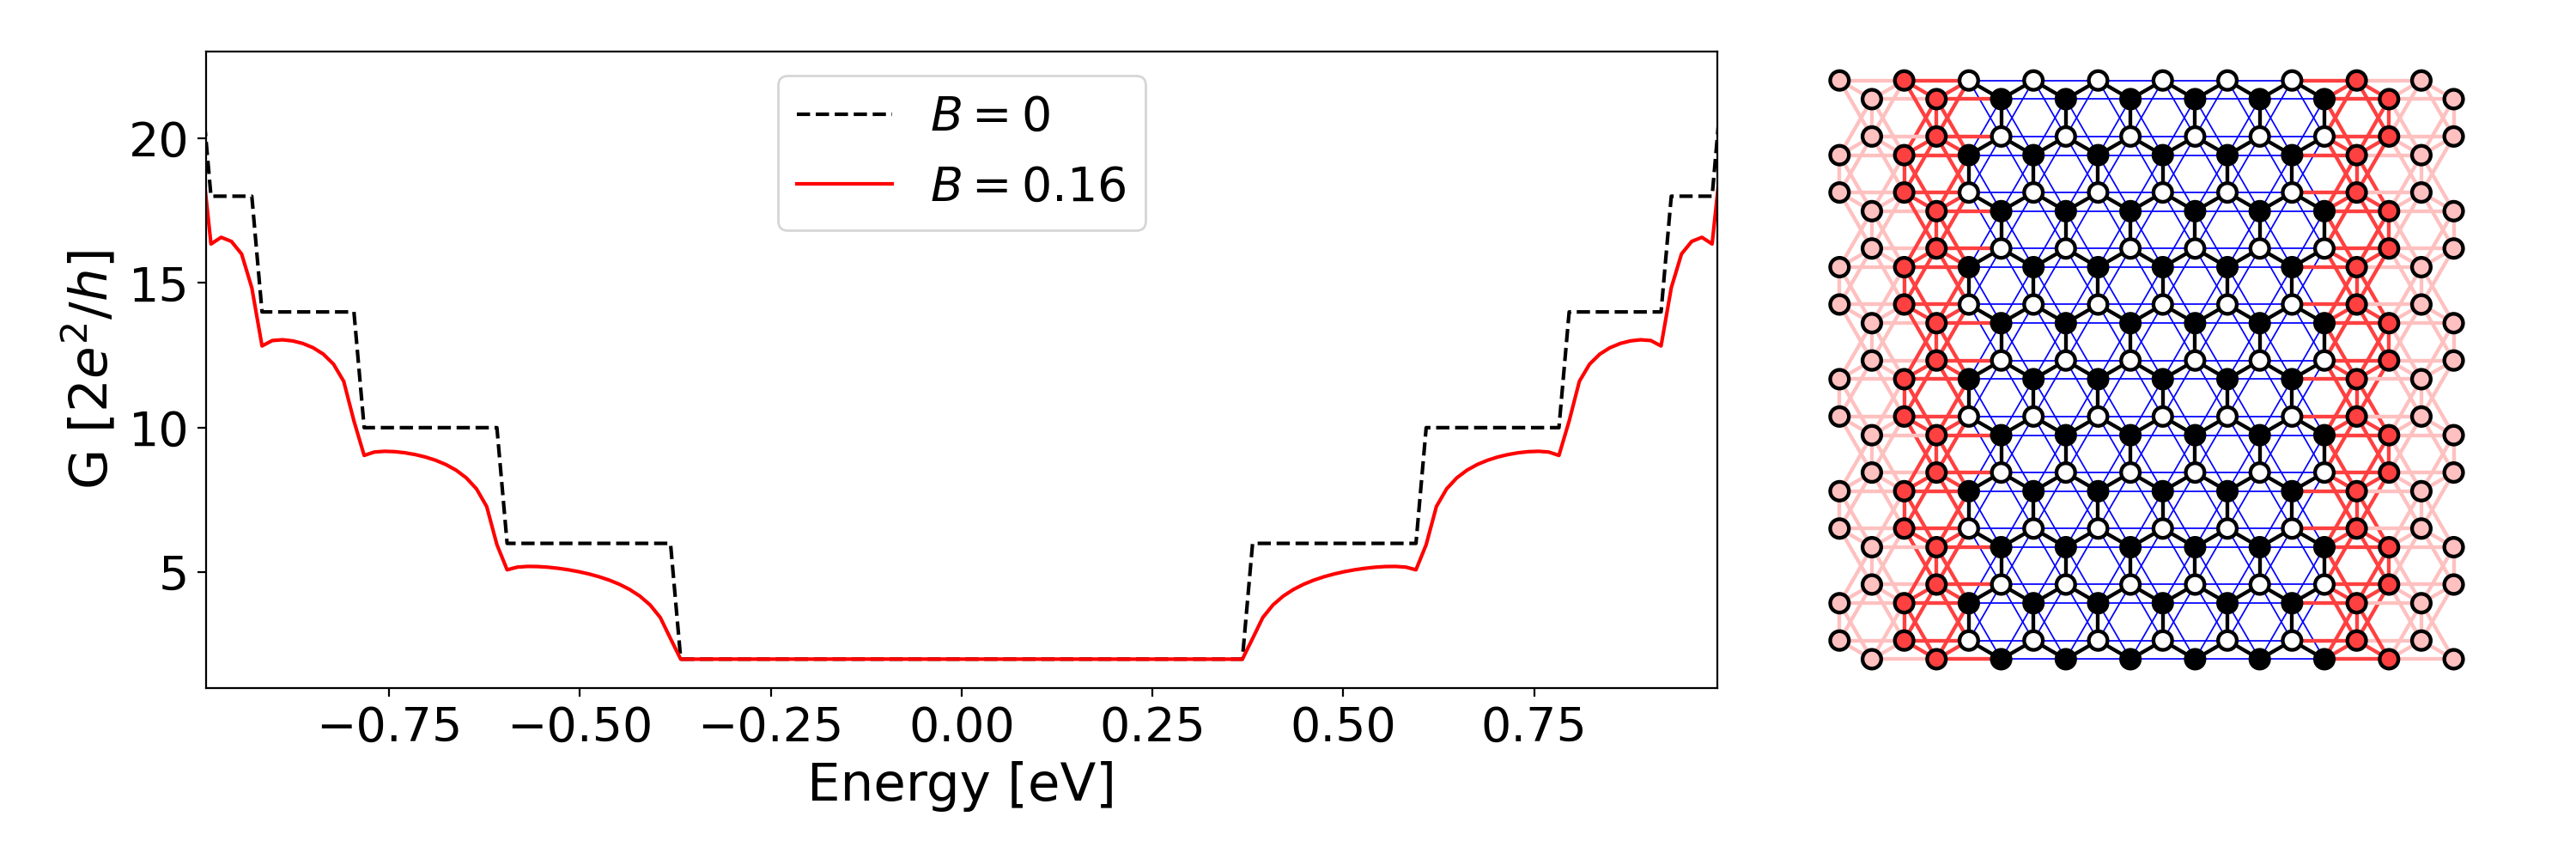
\includegraphics[width=0.9\columnwidth]{/home/marcos/Documents/DAAD_Research/quantum_transport/hydrogenated_graphene/jupyter_notebooks/conductance_wo_adatom_comparison_with_B}
\par\end{centering}
\caption{Comparison between systems with and without magnetic field. }
\end{figure}

\begin{figure}
\begin{centering}
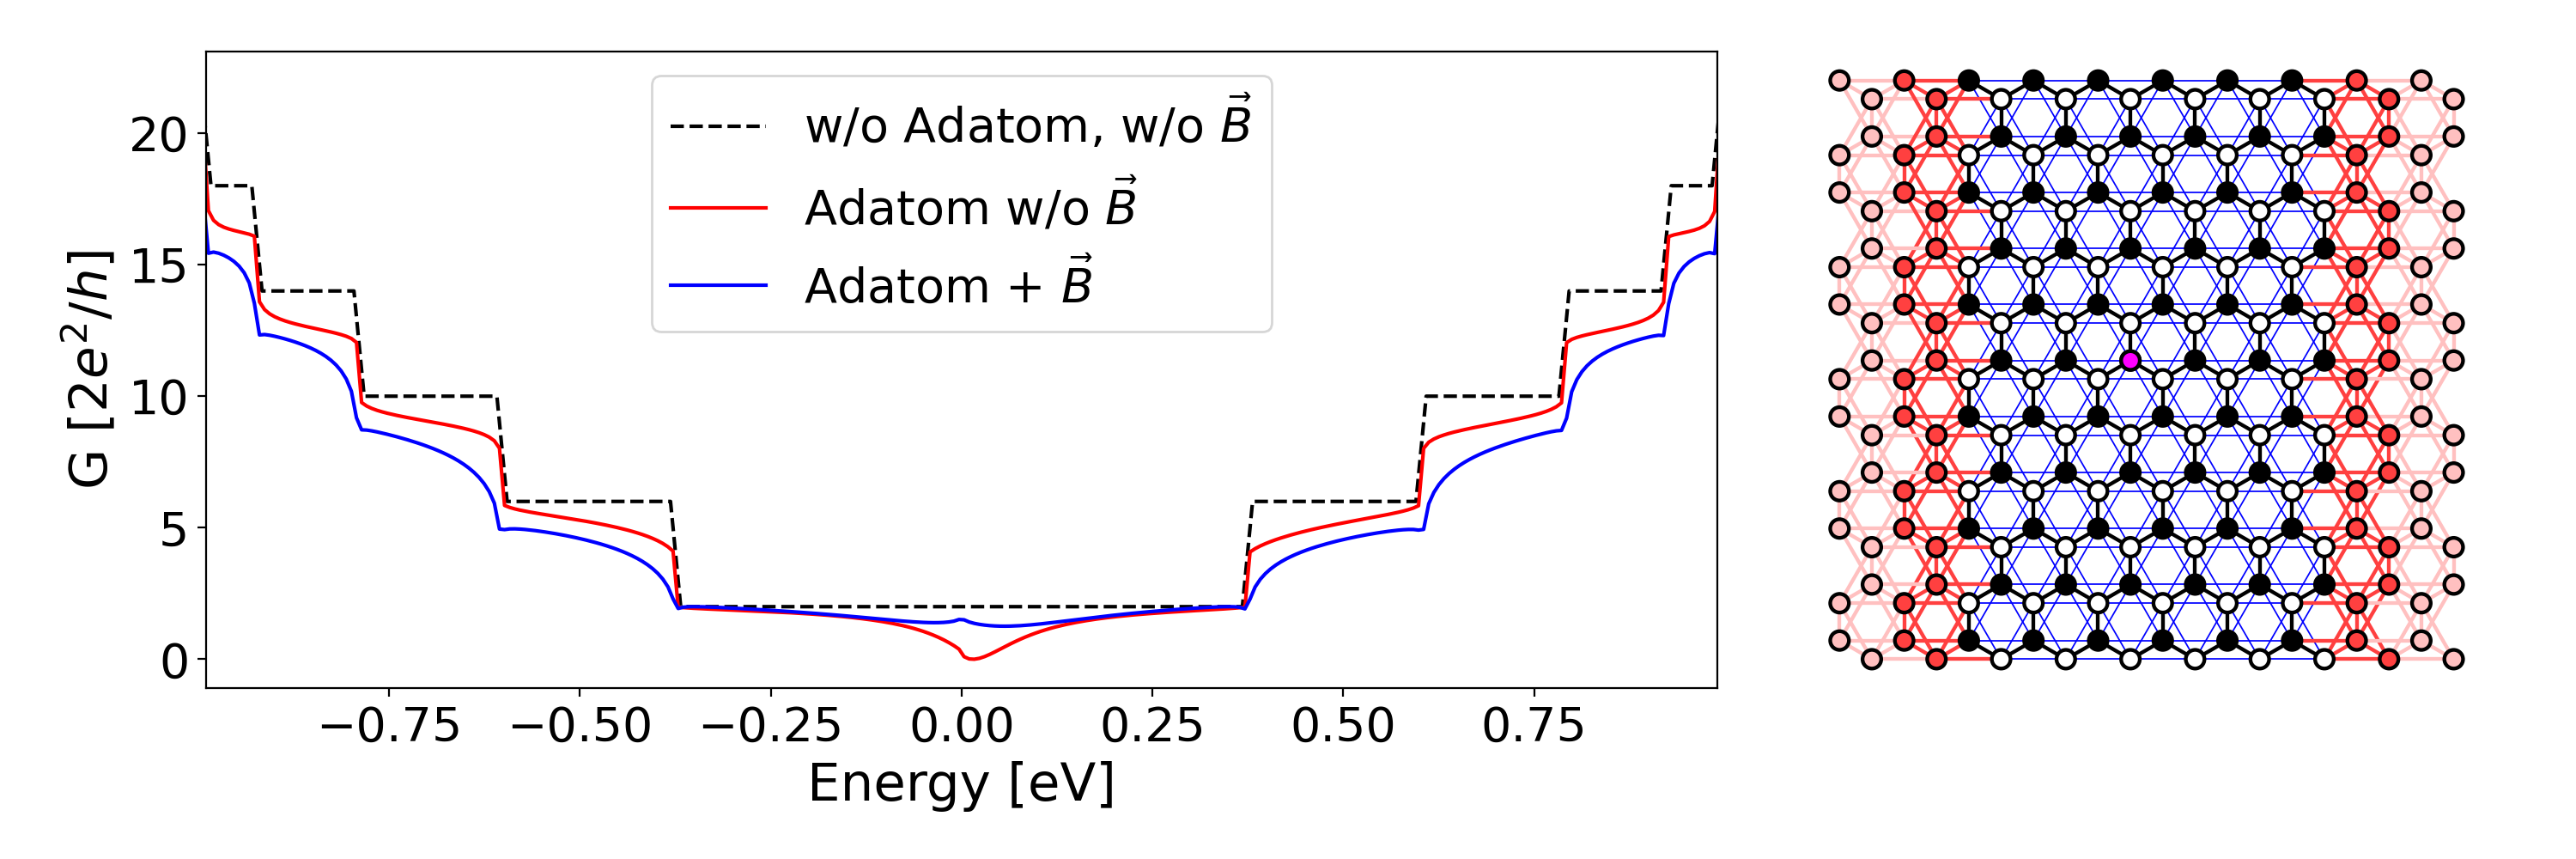
\includegraphics[width=0.9\columnwidth]{/home/marcos/Documents/DAAD_Research/quantum_transport/hydrogenated_graphene/jupyter_notebooks/conductance_with_adatom_comparison_with_B_and_wo_adatom}
\par\end{centering}
\caption{Comparison between systems with a single Adatom in the middle, with
and without magnetic field. }

\end{figure}

\begin{figure}
\begin{centering}
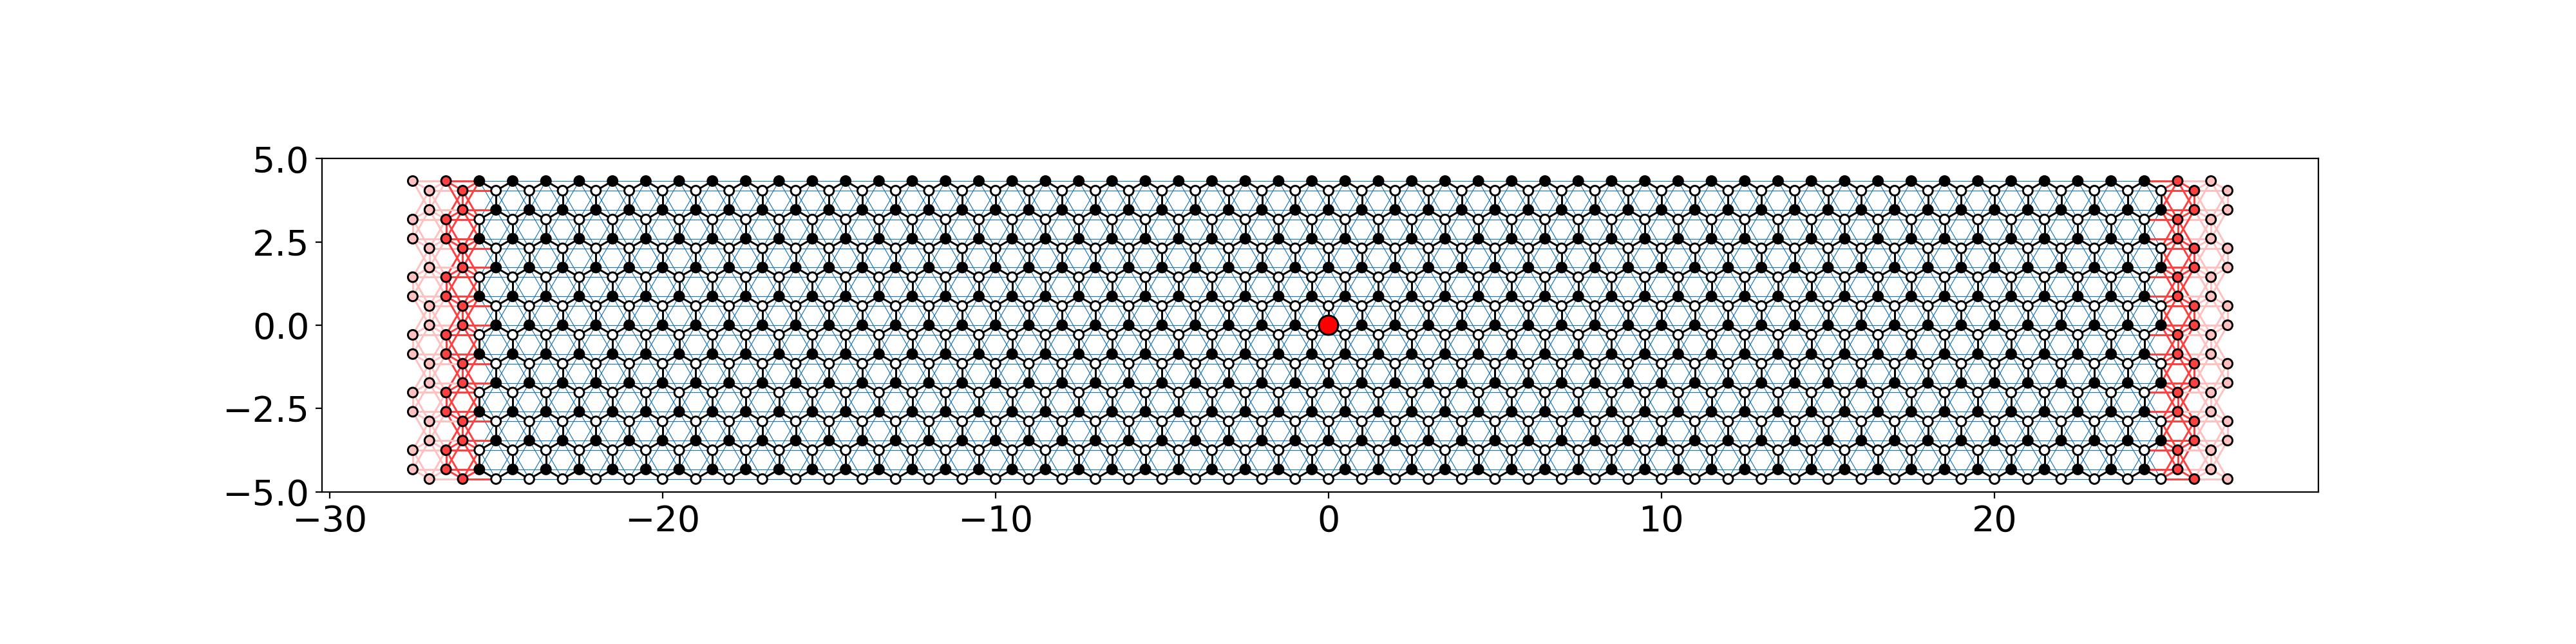
\includegraphics[width=0.9\columnwidth]{/home/marcos/Documents/DAAD_Research/quantum_transport/hydrogenated_graphene/jupyter_notebooks/system_long}
\par\end{centering}
\caption{Representation of the system adopted in the density of states calculations.
Here we have the leads}
\end{figure}

\begin{figure}
\begin{centering}
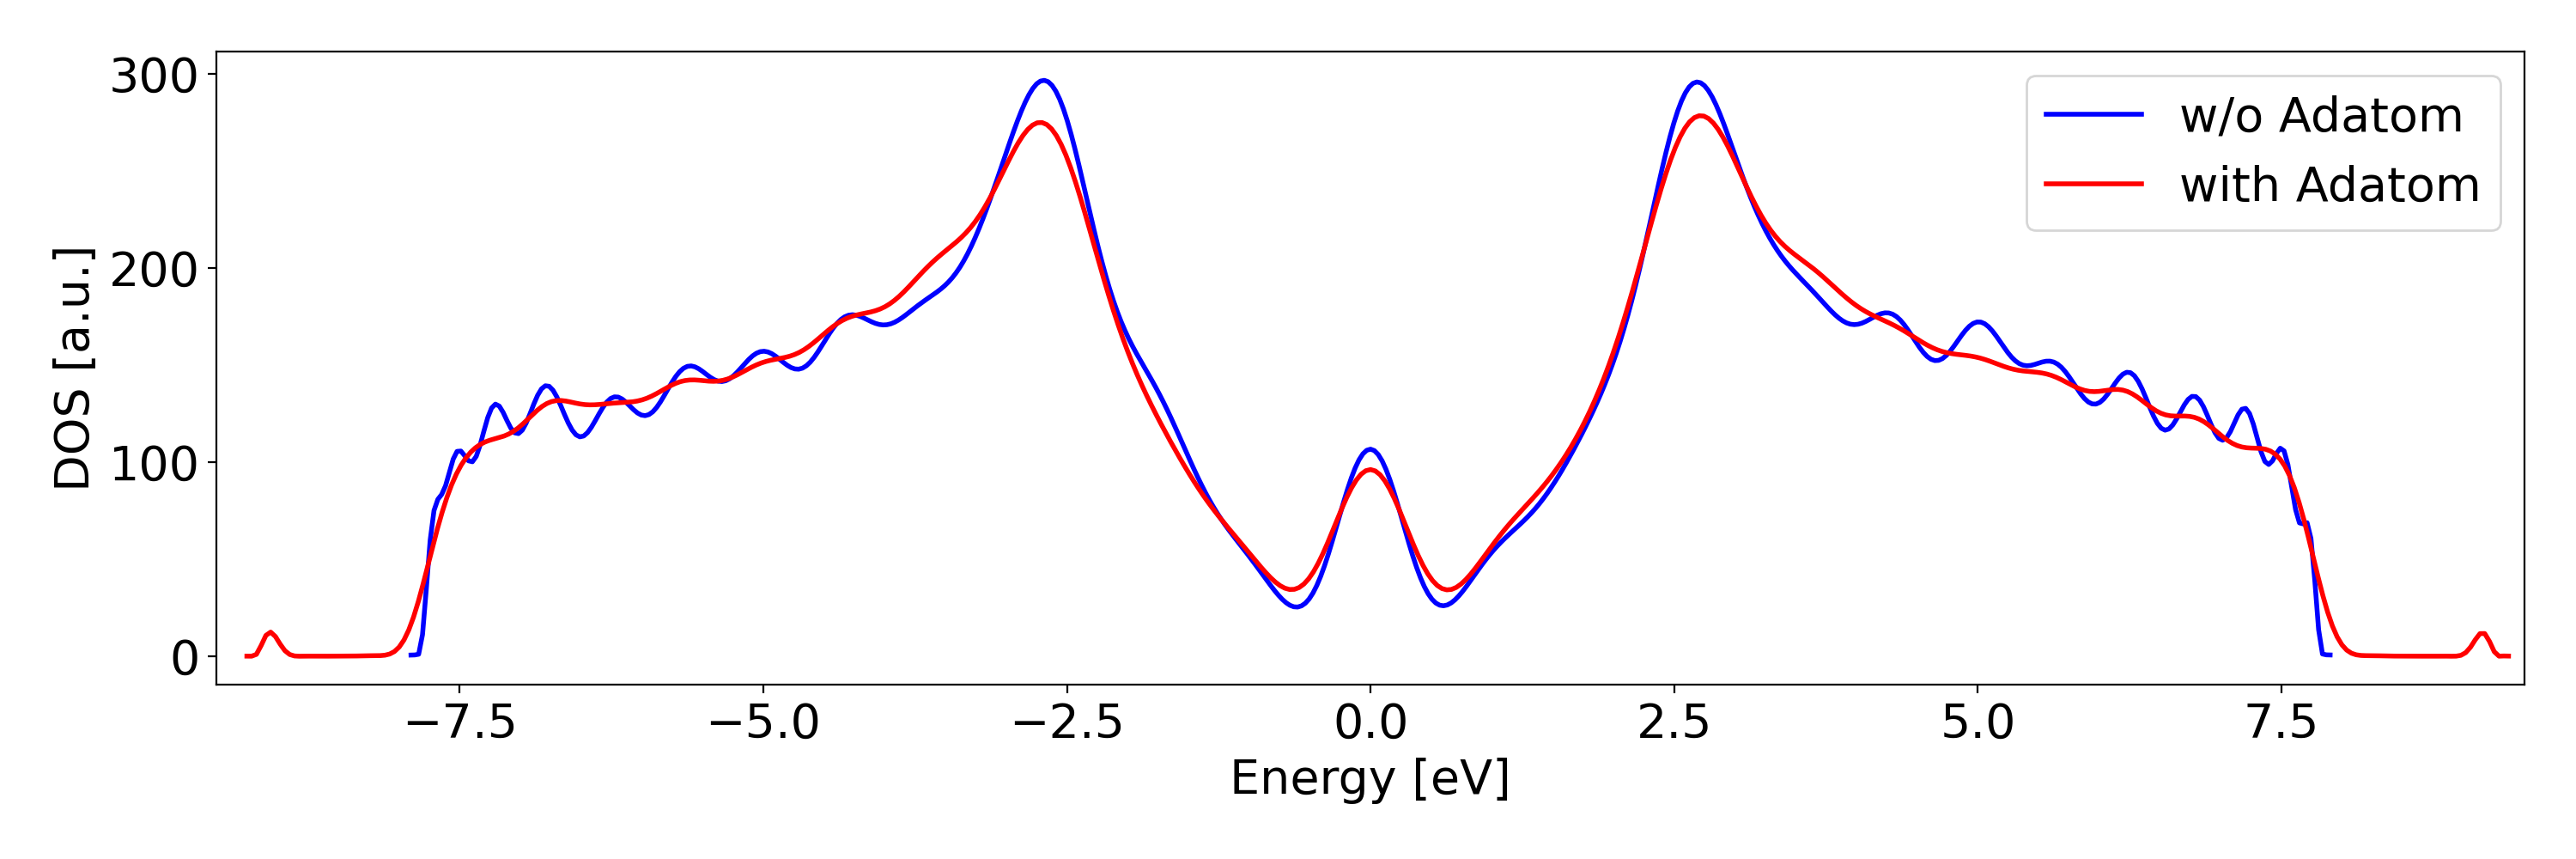
\includegraphics[width=0.8\columnwidth]{/home/marcos/Documents/DAAD_Research/quantum_transport/hydrogenated_graphene/jupyter_notebooks/total_dos_comparison}
\par\end{centering}
\caption{Total density of states comparison between the systems with and withou
the adatom. Both the systems have a rectangular shape and zig zag
bouraries. The adatom was placed on top of the Carbon atom at the
origin of the coordinate system, which is approximately the center
of the system.}

\end{figure}

\begin{figure}
\begin{centering}
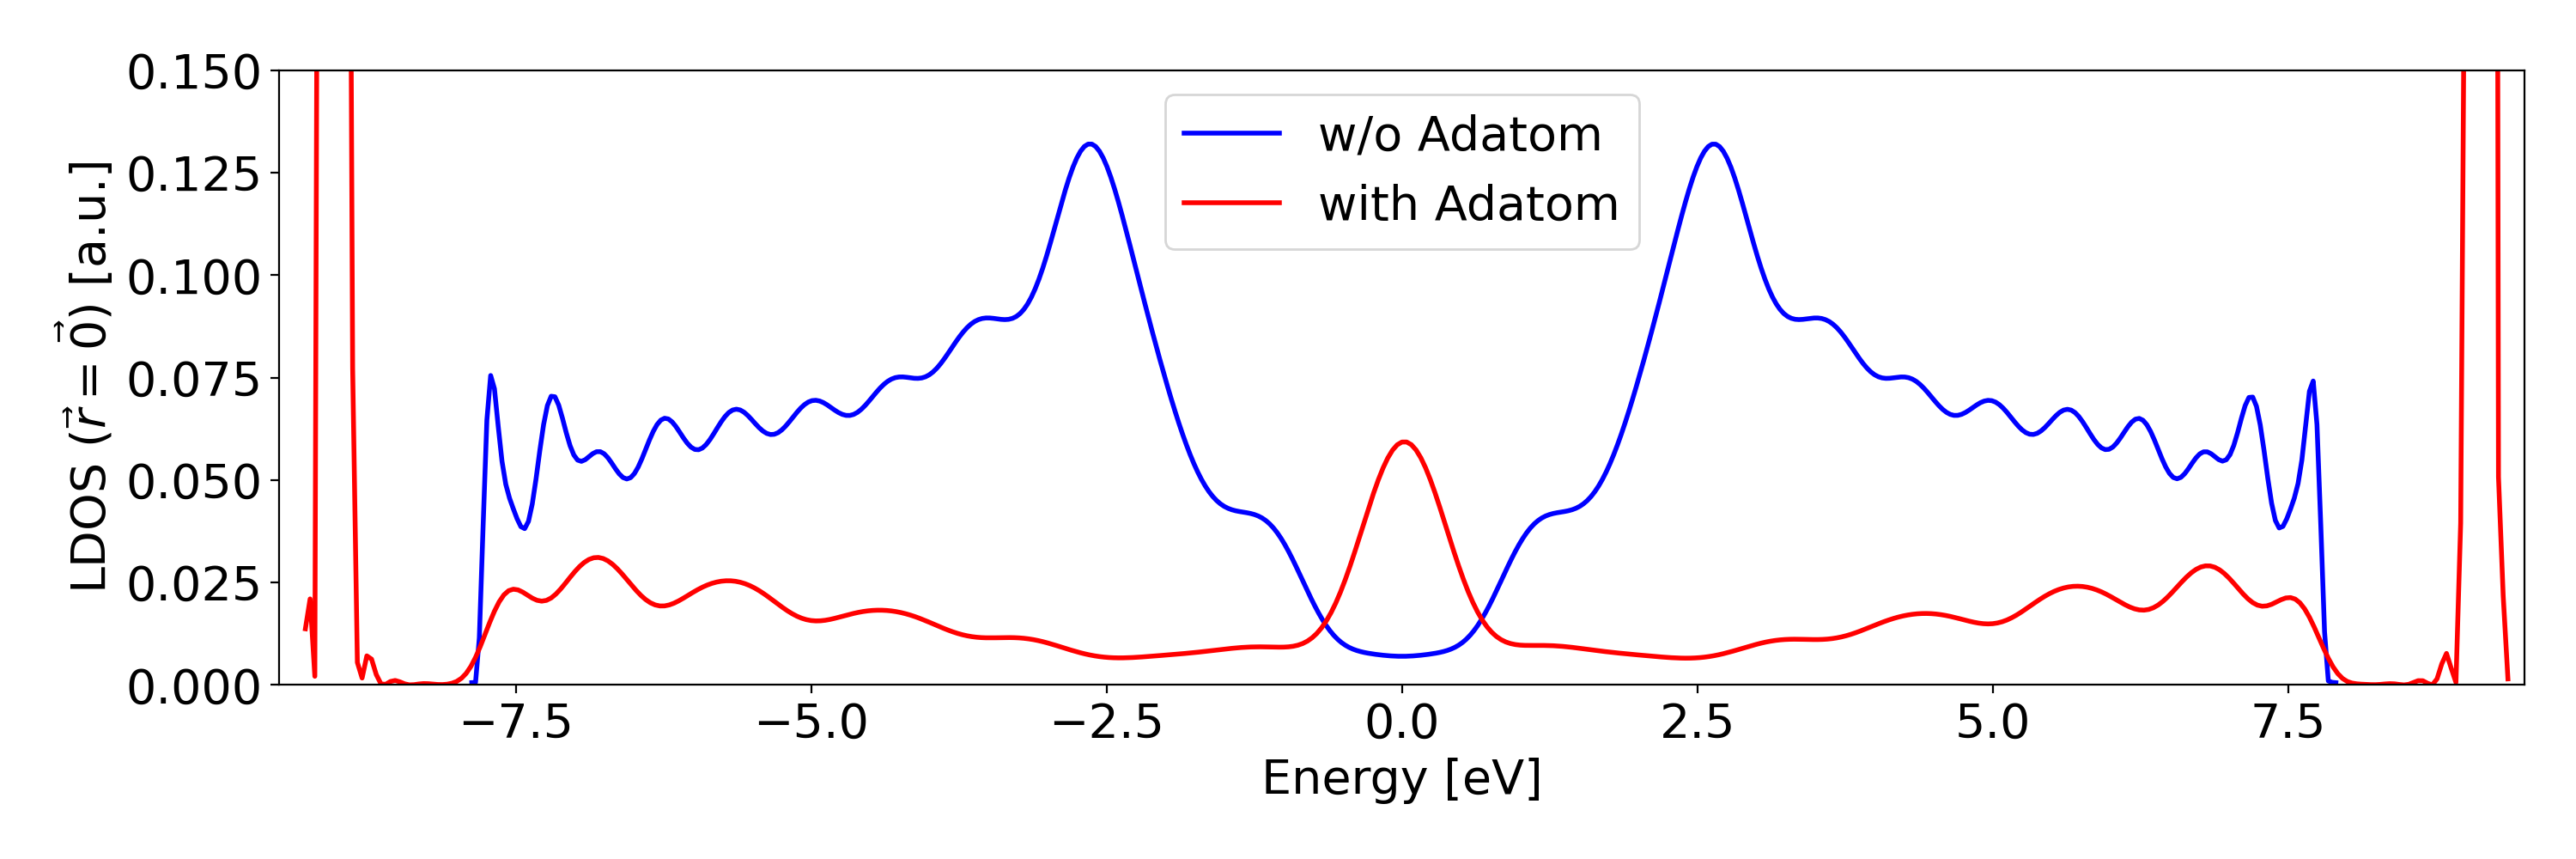
\includegraphics[width=0.9\columnwidth]{/home/marcos/Documents/DAAD_Research/quantum_transport/hydrogenated_graphene/jupyter_notebooks/ldos_at_center_comparison}
\par\end{centering}
\caption{Local density of states (LDOS) for the position $\vec{r}=0$. In blue
we have the results for the system without the adatom while the red
line shows the results for the system with the adatom positioned at
the center. The important features here is the presence of the peak
for energy zero, and the very high peaks at the both ends of the energy
range. }

\end{figure}

\begin{figure}
\begin{centering}
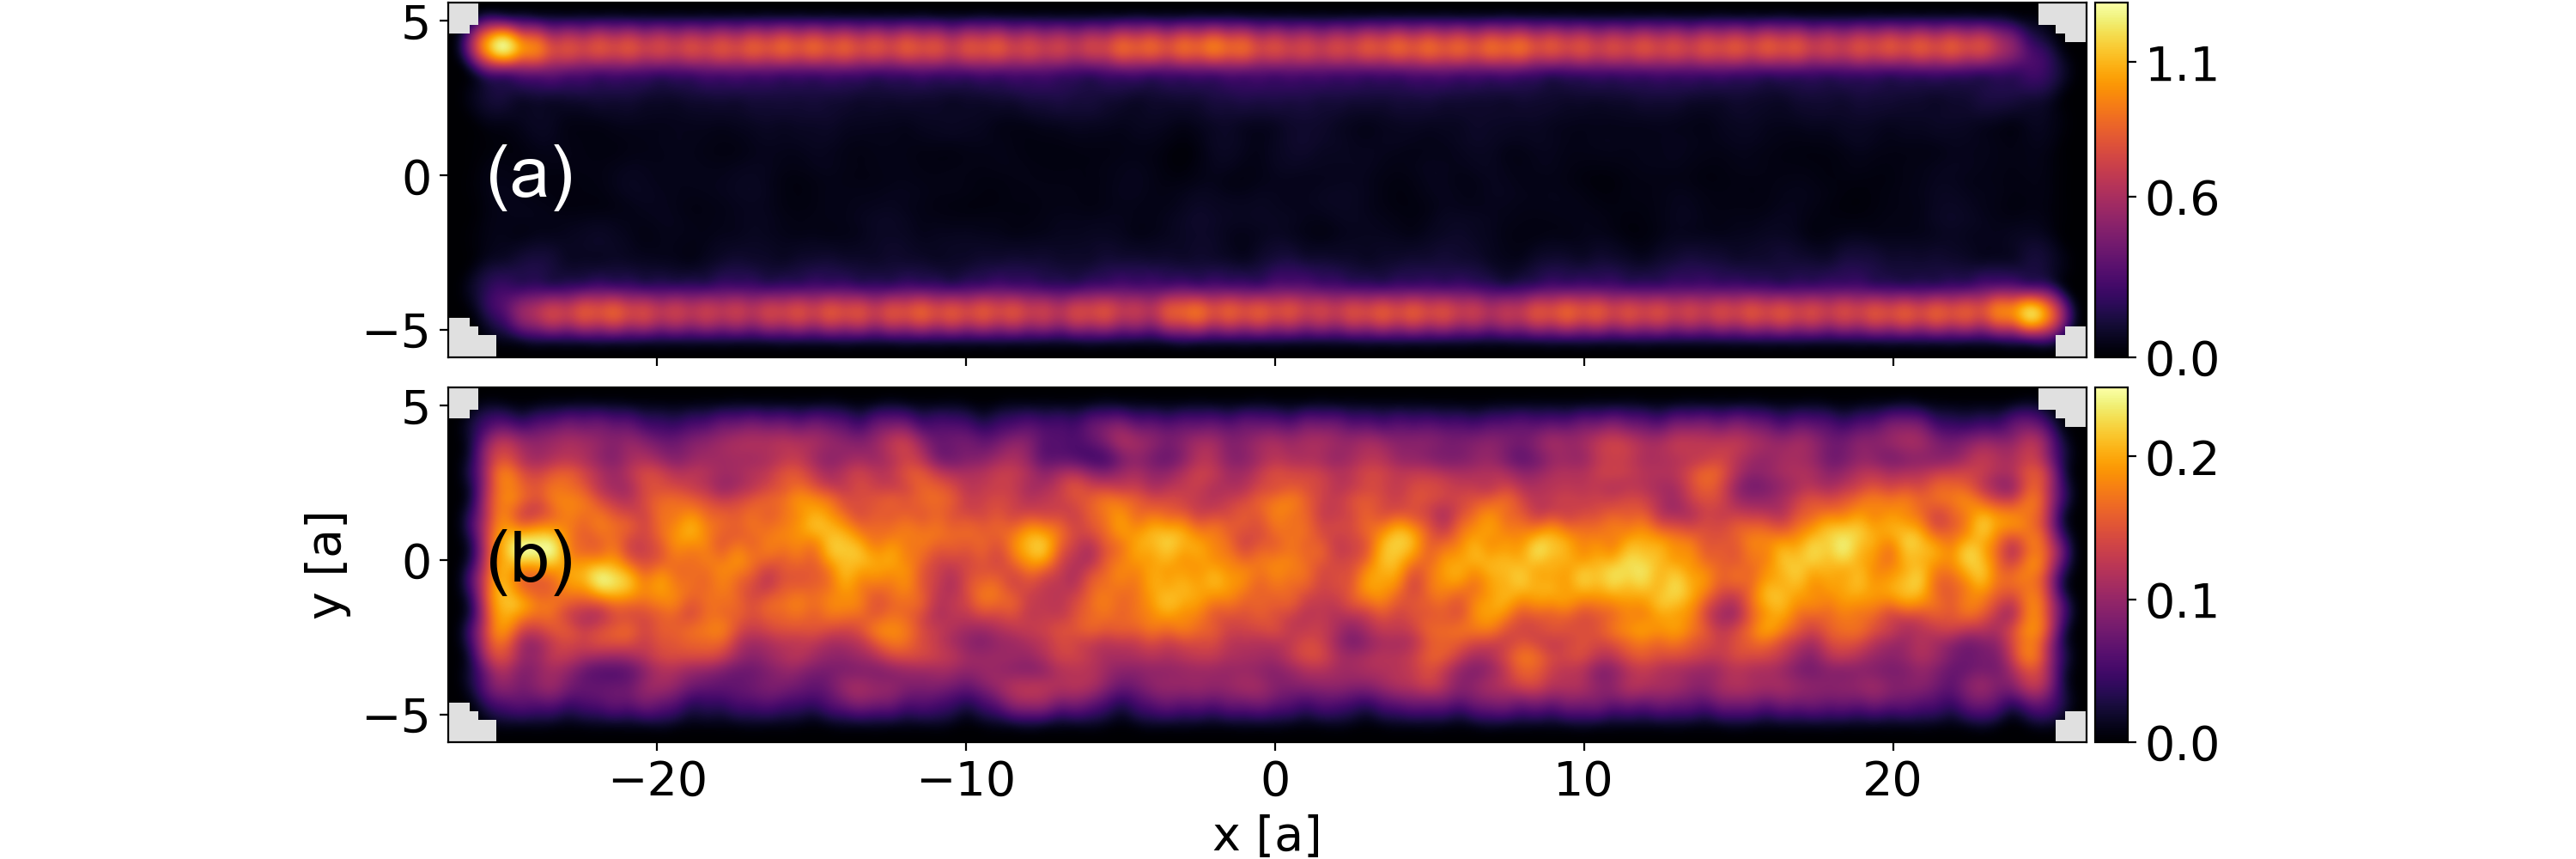
\includegraphics[width=0.9\columnwidth]{/home/marcos/Documents/DAAD_Research/quantum_transport/hydrogenated_graphene/jupyter_notebooks/ldos_E_0_and_E_1_without_adatom}
\par\end{centering}
\caption{Color map for the local density of states for the system without adatom.
In the panel (a) we have the mapping for $E=0$, and in (b) we have
the mapping for the $E=1$ eV. }

\end{figure}

\begin{figure}
\begin{centering}
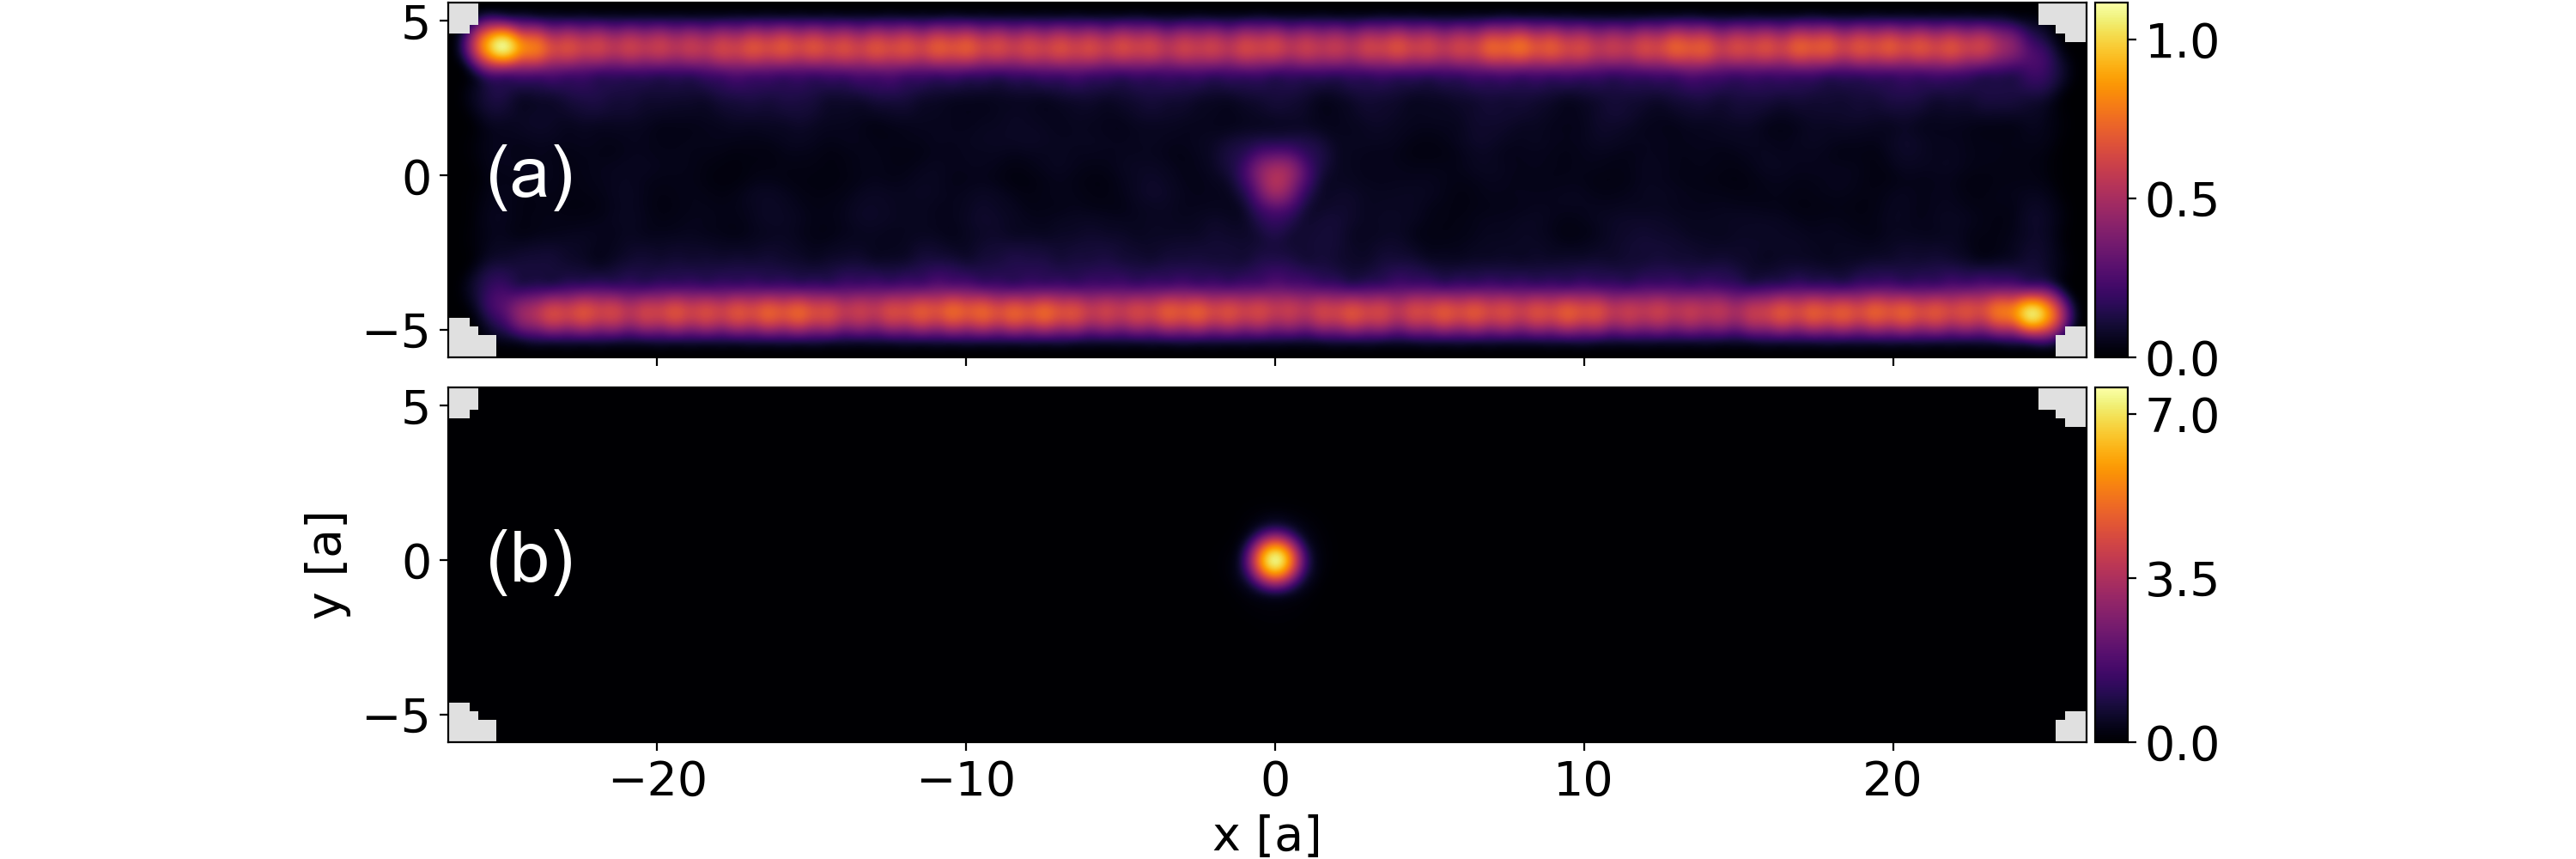
\includegraphics[width=0.9\columnwidth]{/home/marcos/Documents/DAAD_Research/quantum_transport/hydrogenated_graphene/jupyter_notebooks/ldos_E_0_and_E_9,17_with_adatom}
\par\end{centering}
\caption{Local density of states for the system with a Hydrogen adatom in the
center. The panel (a) shows the results for $E=0$, while the panel
(b) presents the mapping for energy corresponding to the highest value
of density $E=9.17$ eV. }

\end{figure}

\begin{figure}
\begin{centering}
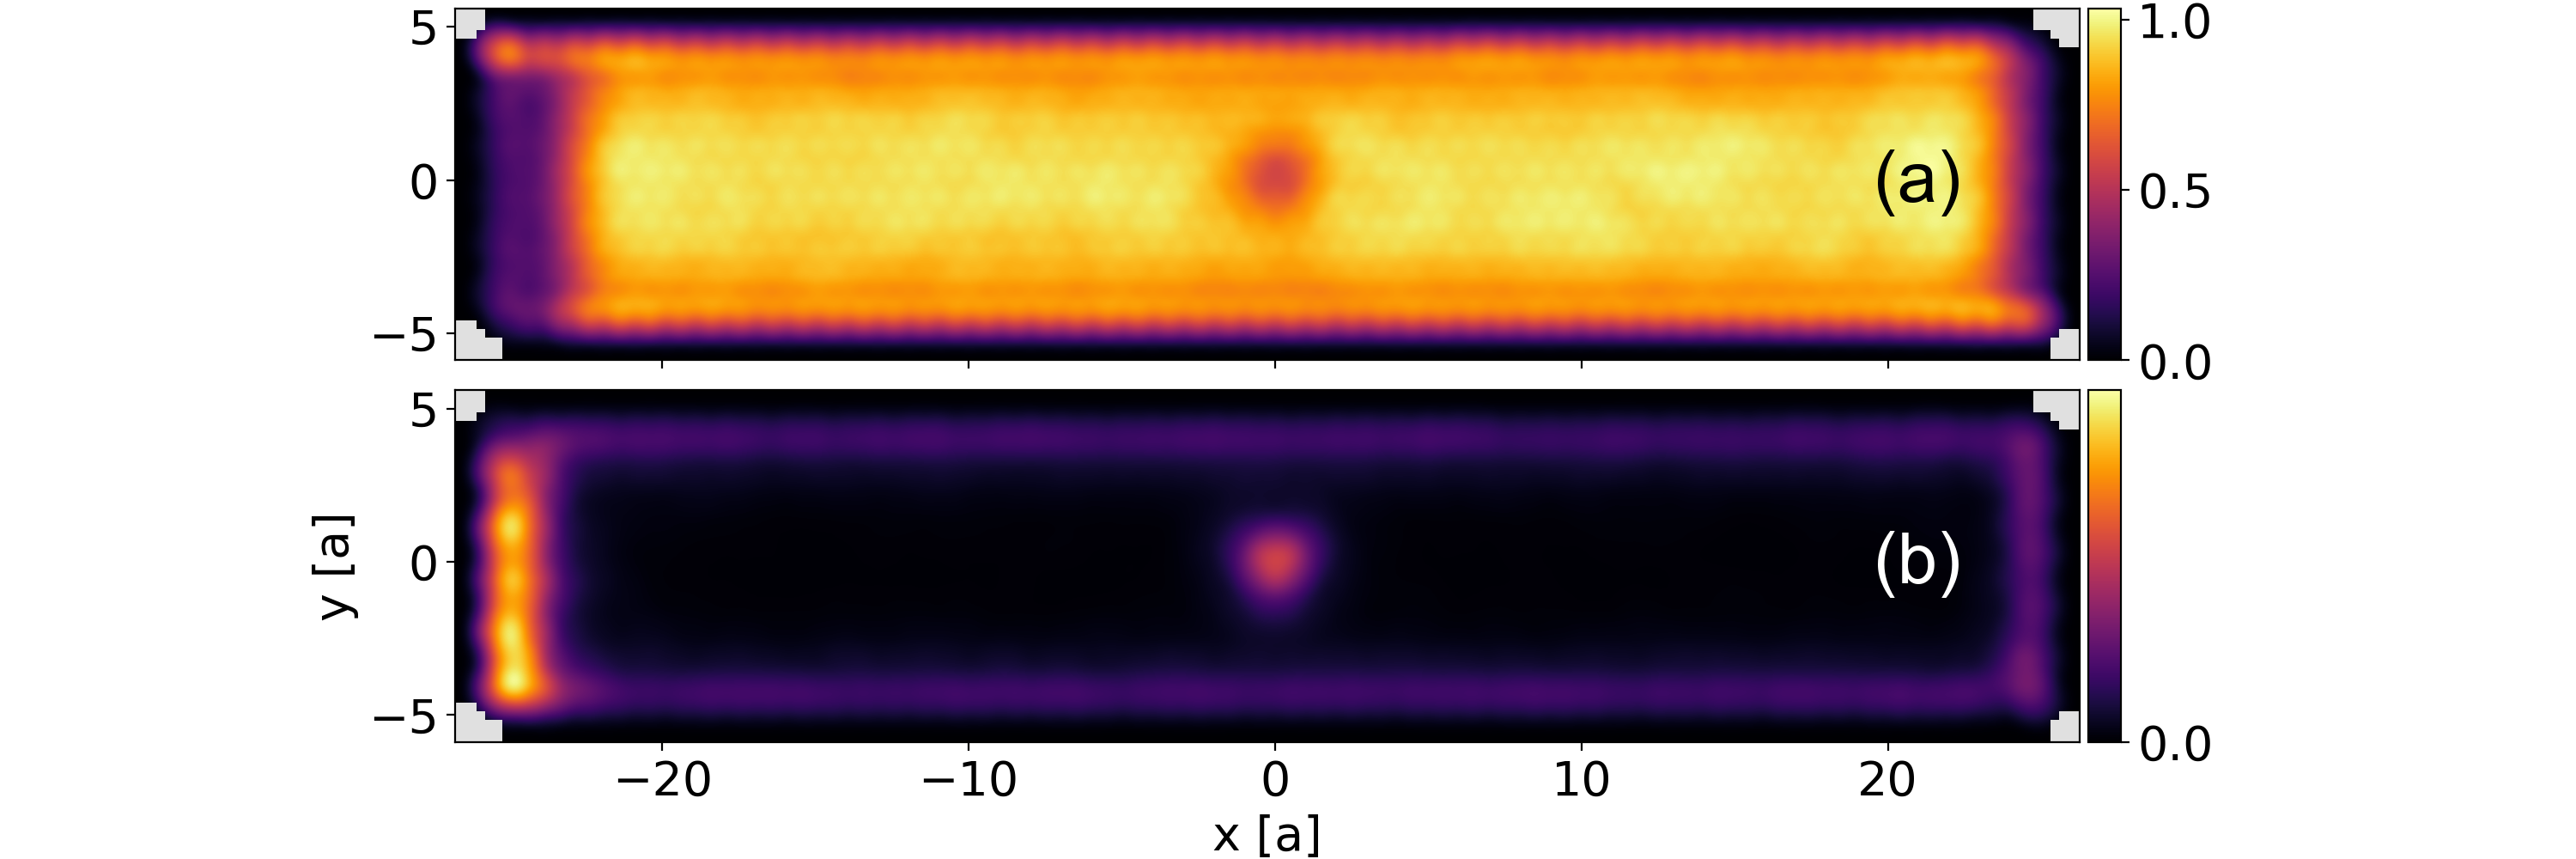
\includegraphics[width=0.9\columnwidth]{/home/marcos/Documents/DAAD_Research/quantum_transport/hydrogenated_graphene/jupyter_notebooks/ldos_E_0_and_E_9,17_adatom_B}
\par\end{centering}
\caption{Local density of states for the system in the presence of magnetic
field.}

\end{figure}


\section{Conclusions}
\end{document}
